% !TEX root = main.tex


%%%%%%%%%%%%%%%%%%%%%%%%%%%%%%%%%%%%%%%%%%%%%%%%%%%%%%%%%%%
\section{Memory model}
\label{memory-model}

Our warm-up example of Section~\ref{symbolic-execution-example} presented a simplified memory model where data are stored in scalar variables only, with no indirection. A crucial aspect of symbolic execution is how memory should be modeled to support programs with pointers and arrays. This requires extending our notion of memory store by mapping not only variables, but also memory addresses to symbolic expressions or concrete values. In general, a store $\sigma$ that explicitly models memory addresses can be thought as a mapping that associates memory addresses (indexes) with either expressions over concrete values or symbolic values. We can still support variables by using their address rather than their name in the mapping. In the following, when we write $x\mapsto e$ for a variable $x$ and an expression $e$ we mean $\&x\mapsto e$, where $\&x$ is the concrete address of variable $x$. Also, if $v$ is an array and $c$ is an integer constant, by $v[c]\mapsto e$ we mean $\&v+c\mapsto e$. A memory model is an important design choice for a symbolic engine, as it can have a significant influence on the coverage achieved by symbolic execution, as well as on the scalability of constraint solving~\cite{CS-CACM13}.

The {\em symbolic memory address} problem~\cite{SAB-SP10} arises when the address referenced in the operation is a symbolic expression. In the remainder of this section, we discuss a number of popular solutions.

\subsection{Fully Symbolic Memory}
\label{ss:fully-symbolic-memory}

At the highest level of generality, an engine may treat memory addresses as fully symbolic. This is the approach taken by a number of works (e.g., {\sc BitBlaze}~\cite{BITBLAZE-ICISS08},~\cite{TLL-CAV10}, {\sc BAP}~\cite{BAP-CAV11}, and~\cite{TS-ATVA14}). Two fundamental approaches, pioneered by King in its seminal paper~\cite{K-CACM76}, are the following:

\begin{itemize}

\item {\em State forking.} If an operation reads from or writes to a symbolic address, the state is forked by considering all possible states that may result from the operation. The path constraints are updated accordingly for each forked state.
\boxedexample{Consider the code shown in Figure~\ref{fi:example-mem}. The write operation at line 4 affects either $a[0]$ or $a[1]$, depending on the unknown value of array index $i$. State forking creates two states after executing the memory assignment to explicitly consider both possible scenarios (Figure~\ref{fi:memory-fork}). The path constraints for the forked states encode the assumption made on the value of $i$. Similarly, the memory read operation \texttt{a[j]} at line 5 may access either $a[0]$ or $a[1]$, depending on the unknown value of array index $j$. Therefore, for each of the two possible outcomes of the assignment \texttt{a[i]=5}, there are two possible outcomes of the \texttt{assert}, which are explicitly explored by forking the corresponding states. }

\begin{figure}[ht]
\begin{center}
\begin{tabular}{c}
\begin{lstlisting}[basicstyle=\ttfamily\scriptsize]
1.  void foobar(unsigned i, unsigned j) {
2.     int a[2] = { 0 };
3.     if (i>1 || j>1) return;
4.     a[i] = 5;
5.     assert(a[j] != 5);
6.  }
\end{lstlisting}
\end{tabular}
\end{center}
\vspace{-2mm}
\caption{Memory modeling example: which values of \texttt{i} and \texttt{j} make the \texttt{assert} fail?}
\label{fi:example-mem}
\end{figure}

\begin{figure}[ht]
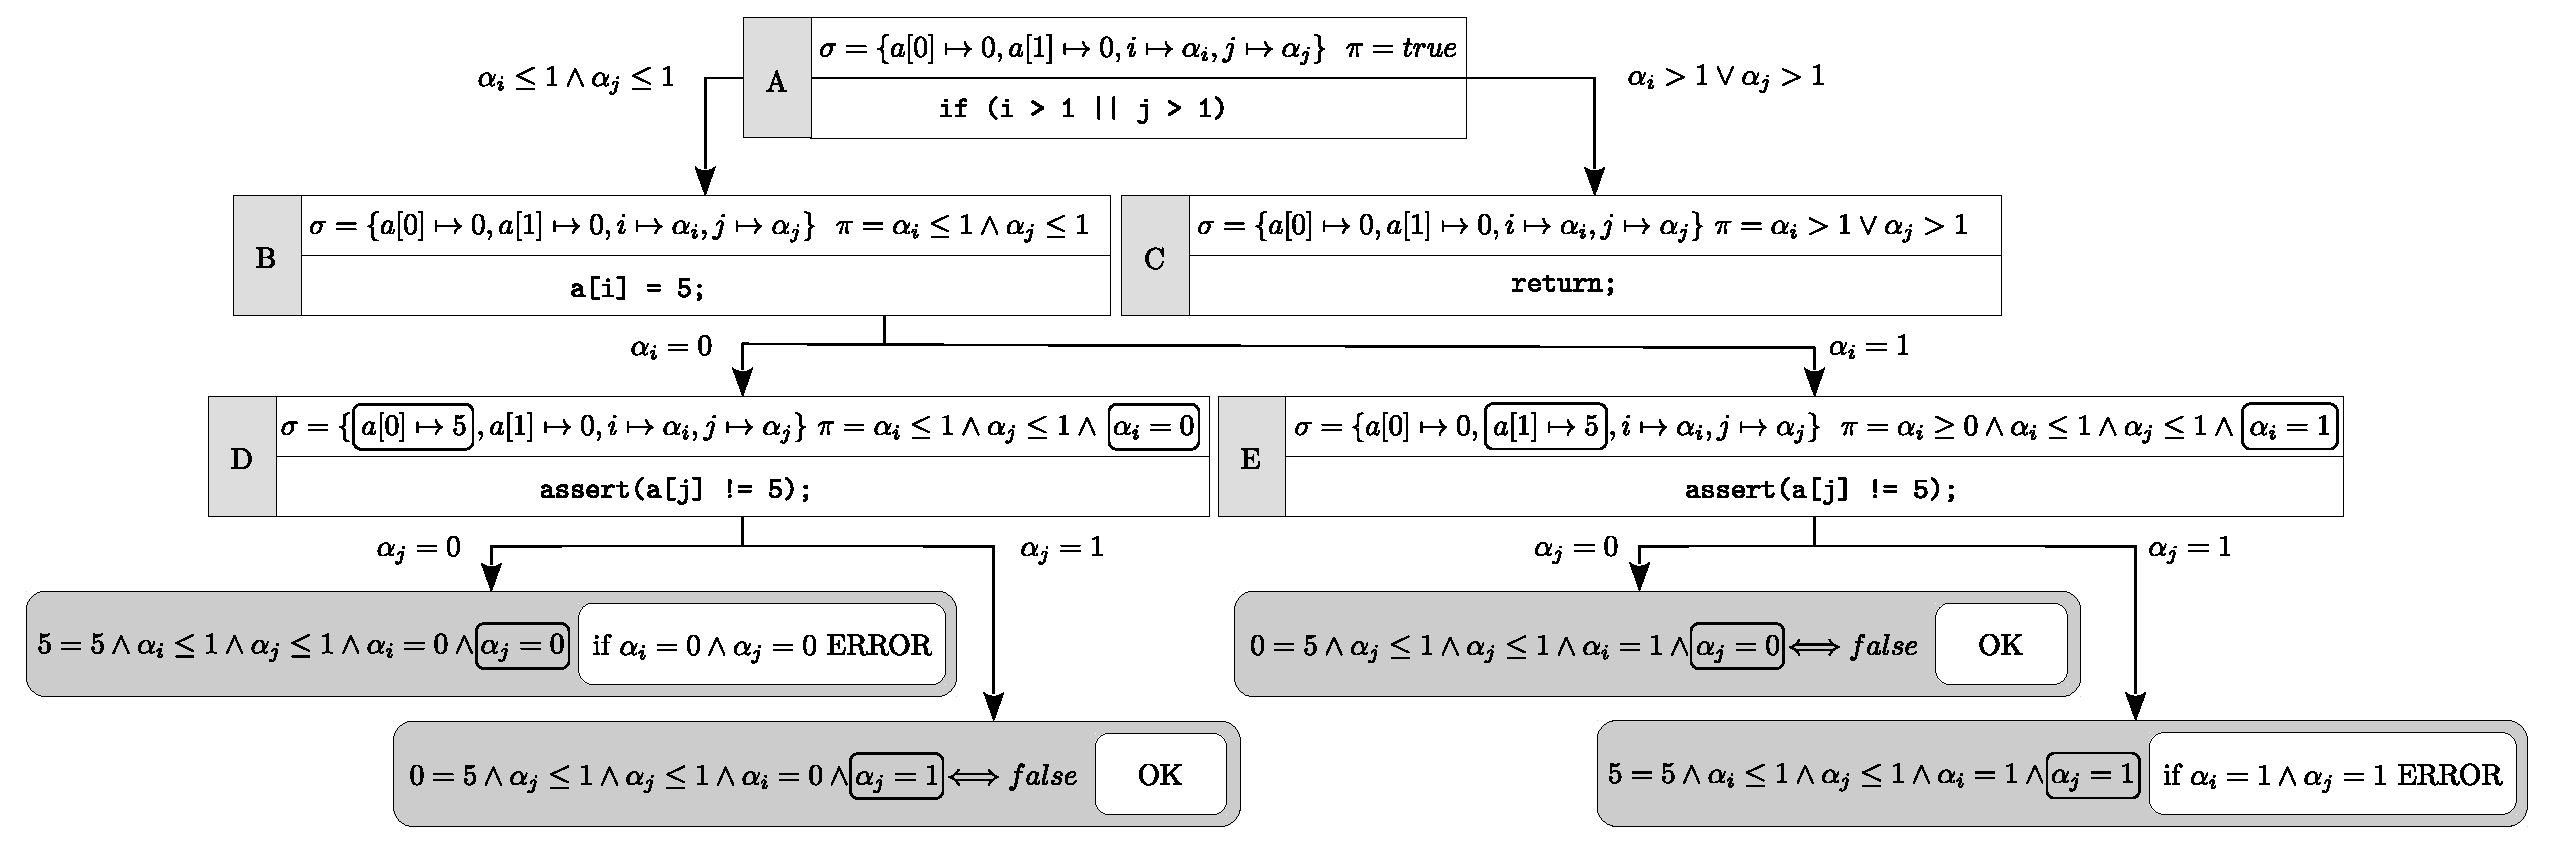
\includegraphics[width=1\columnwidth]{images/memory-fork} 
\vspace{-4.5mm}
\caption{Fully symbolic memory via state forking for the example of Figure~\ref{fi:example-mem}.}
\label{fi:memory-fork}
\end{figure}

\item {\em if-then-else formulas.} An alternative approach consists in encoding the uncertainty on the possible values of a symbolic pointer into the expressions kept in the symbolic store and in the path constraints, without forking any new states. The key idea is to exploit the capability of some solvers to reason on formulas that contain if-then-else expressions of the form $ite(\texttt{c}, \texttt{t}, \texttt{f})$, which yields \texttt{t} if \texttt{c} is true, and \texttt{f} otherwise\footnote{In propositional logic, the $ite(\texttt{c}, \texttt{t}, \texttt{f})$ expression could be replaced with the formula $(\texttt{c} \wedge \texttt{t}) \vee (\neg\texttt{c} \wedge \texttt{f})$.}.
The approach works differently for memory read and write operations. Let $\alpha$ be a symbolic address that may assume the concrete values $a_1, a_2, \ldots$:
\begin{itemize}
\item reading from $\alpha$ yields the expression $ite(\alpha=a_1,\sigma(a_1), ite(\alpha=a_2,\sigma(a_2), \ldots))$;
\item writing an expression $e$ at $\alpha$ updates the symbolic store for each $a_1, a_2, \ldots$ as $\sigma(a_i)\gets ite(\alpha=a_i,e,\sigma(a_i))$.
\end{itemize}
Notice that in both cases, a memory operation introduces in the store as many $ite$ expressions as the number of possible values the accessed symbolic address may assume. The $ite$ approach to symbolic memory is used, e.g., in {\sc Angr}~\cite{ANGR-SSP16} (Section~\ref{ss:index-based-memory}).
\boxedexample{Consider again the example shown in Figure~\ref{fi:example-mem}. Rather than forking the state after the operation \texttt{a[i]=5} at line 4, the if-then-else approach updates the memory store by encoding both possible outcomes of the assignment, i.e., $a[0]\mapsto ite(\alpha_i=0,5,0)$ and $a[1]\mapsto ite(\alpha_i=1,5,0)$ (Figure~\ref{fi:memory-ite}). Similarly, rather than creating a new state for each possible distinct address of \texttt{a[j]} at line 5, the uncertainty on $j$ is encoded in the single expression $ite(\alpha_j=0,\sigma(a[0]),\sigma(a[1]))=ite(\alpha_j=0,ite(\alpha_i=0,5,0),ite(\alpha_i=1,5,0))$.
%: if $\alpha_i=0$ then $a[0]\mapsto 5$ and $a[1]\mapsto 0$; conversely, if $\alpha_i=1$ then $a[0]\mapsto 0$ and $a[1]\mapsto 5$.
%State forking creates two states after executing the memory assigment to explicitly consider both possible scenarios (Figure~\ref{fi:memory-fork}). The path constraints for the forked states encode the assumption made on the value of $i$. Similarly, the memory read operation \texttt{a[j]} at line 5 may access either $a[0]$ or $a[1]$, depending on the unknown value of array index $j$. Therefore, for each of the two possible outcomes of the assignment \texttt{a[i]=5}, there are two possible outcomes of the \texttt{assert}, which are explicitly explored by forking the corresponding states. 
}

%Indeed, the $ite(\texttt{c}, \texttt{t}, \texttt{f})$ expression introduced in the symbolic store $\sigma$ is a short term for an {\tt if-then-else} expression and means that if the condition {\tt c} is verified then {\tt t} holds, otherwise {\tt f} must be assumed as true. Nonetheless, $ite$ expressions are often just syntactic sugar for disjunctive formulas and are commonly supported by most prominent constraint solvers. For instance, in the context of propositional logic the $ite(\texttt{c}, \texttt{t}, \texttt{f})$  expression could be replaced with the formula $(\texttt{c} \wedge \texttt{t}) \vee (\neg\texttt{c} \wedge \texttt{f})$ . 

\end{itemize}

\begin{figure}[t]
\begin{center}
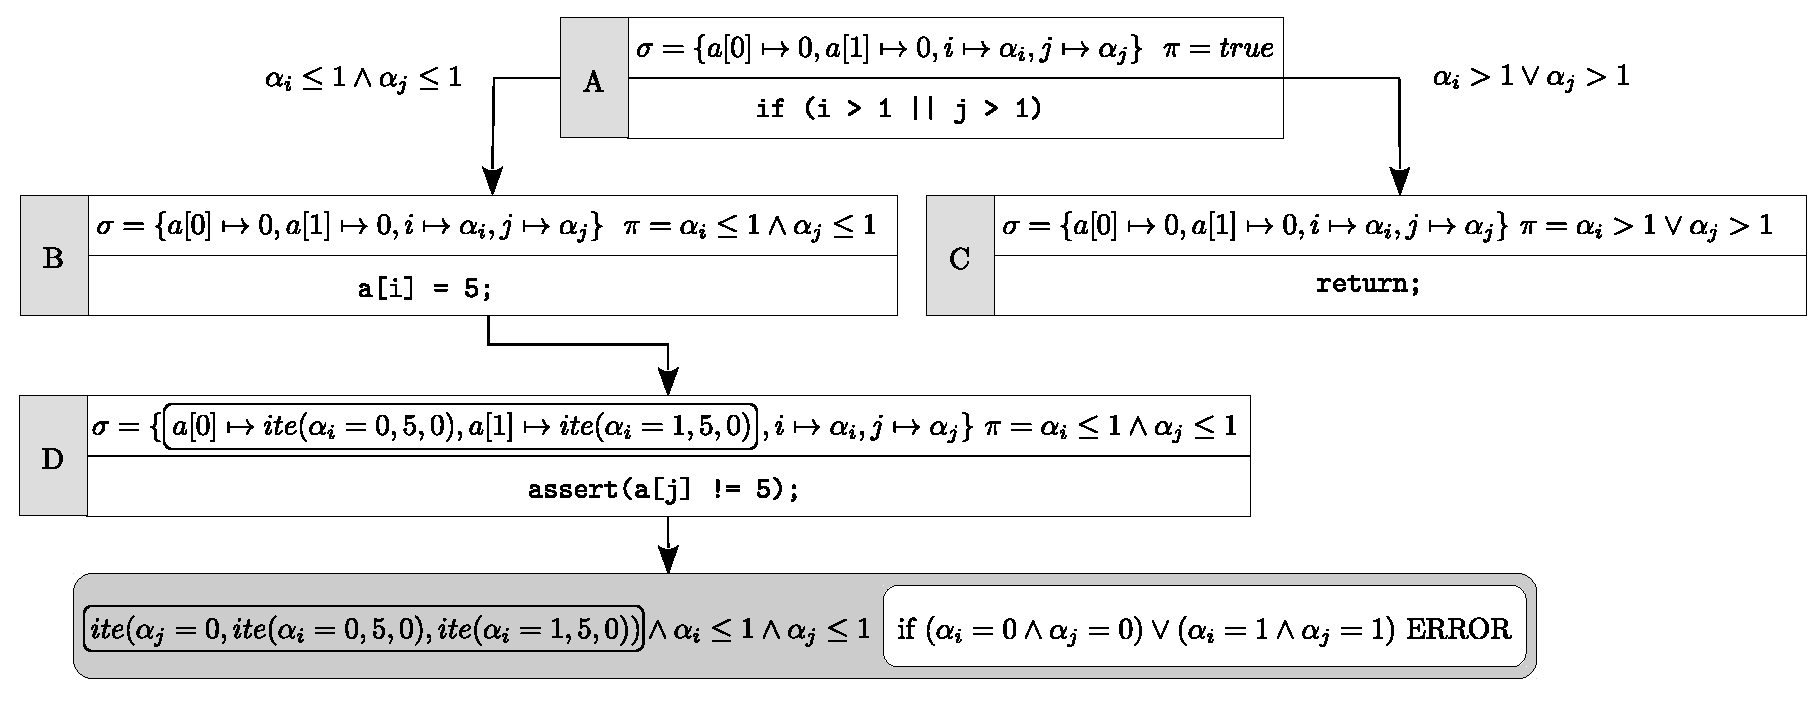
\includegraphics[width=0.7\columnwidth]{images/memory-ite} % TODO 0.7
\end{center}
\vspace{-2.5mm}
\caption{Fully symbolic memory via if-then-else formulas for the example of Figure~\ref{fi:example-mem}.}
%\vspace{-1mm} % TODO
\label{fi:memory-ite}
\end{figure}

%\noindent To model fully symbolic pointers, an extensive line of research (e.g., {\sc EXE}~\cite{EXE-CCS06}, {\sc KLEE}~\cite{KLEE-OSDI08}, {\sc SAGE}~\cite{EGL-ISSTA09}) leverages the expressive power of SMT solvers to model array operations as first-class entities in constraint formulas using a {\em theory of arrays} in the decision procedure~\cite{STP-CAV07}.

\noindent \mynote{[D] rephrased} An extensive line of research (e.g., {\sc EXE}~\cite{EXE-CCS06}, {\sc KLEE}~\cite{KLEE-OSDI08}, {\sc SAGE}~\cite{EGL-ISSTA09}) leverages the expressive power of some SMT solvers to model fully symbolic pointers. Using a {\em theory of arrays}~\cite{STP-CAV07}, array operations can in fact be expressed as first-class entities in constraint formulas.

\mytempedit{
Due to its generality, fully symbolic memory supports the most accurate description of the memory behavior of a program, accounting for all possible memory manipulations. In many practical scenarios, the set of possible addresses a memory operation may reference is small~\cite{BITBLAZE-ICISS08} as in the example shown in Figure~\ref{fi:example-mem} where indexes $i$ and $j$ range in a bounded interval, allowing accurate analyses using a reasonable amount of resources. In general, however, a symbolic address may reference any cell in memory, leading to an intractable explosion in the number of possible states. For this reason, a number of techniques have been designed to improve scalability, which fall into three main categories:

\begin{itemize}

\item {\em Representing memory in a compact form.} This approach was taken in~\cite{MEMSIGHT-ASE17}, which maps symbolic -- rather than concrete -- address expressions to data, maintaining the possible alternative states resulting from the memory referenced by a symbolic address in a compact, implicit form. Queries are offloaded to efficient paged interval tree implementations to determine which stored data are possibly referenced by a memory read operation.

\item {\em Trading soundness for performance.} The idea, discussed in Section~\ref{ss:address-concretization} and Section~\ref{ss:index-based-memory}, consists in corseting symbolic exploration to a subset of the execution states by replacing symbolic pointers with concrete addresses.

\item {\em Leveraging language-specific features.} Differently from languages with arbitrary memory access, such as C or assembly, references in object-oriented languages can be assumed to be either null or point to previously allocated objects, rather than to any generic memory location. This allows significantly reducing the exploration space in symbolic execution as discussed in Section~\ref{ss:complex-objects}.

\end{itemize}
}

%When obtained ranges are too large, {\sc BitBlaze}~\cite{BITBLAZE-ICISS08} adds a further constraint to the system to limit its size. However, the authors observe that most symbolic memory accesses are typically already constrained to small ranges in practice, making it unnecessary.

%\vspace{-2pt} % TODO
\subsection{Address Concretization}
\label{ss:address-concretization}

In all cases where the combinatorial complexity of the analysis explodes as pointer values cannot be bounded to sufficiently small ranges, {\em address concretization}, which consists in concretizing a pointer to a single specific address, is a popular alternative. This can reduce the number of states and the complexity of the formulas fed to the solver and thus improve running time, although may cause the engine to miss paths that, for instance, depend on specific values for some pointers. 

%\mynote{DART is mentioned in CS-CACM13 as  using theories of arrays} --> added to the list above.
Concretization arises naturally in offline executors (Section~\ref{ss:principles}). Prominent examples are {\sc DART}~\cite{DART-PLDI05} and early {\sc SAGE} releases~\cite{SAGE-NDSS08} that concretely execute one path at a time while collecting path constraints along executed paths. %\mynote{[D] was: equality and inequality}  
Systems such as {\sc CUTE}~\cite{CUTE-FSE05} and {\sc CREST}~\cite{CREST-ASE08} are capable of reasoning only about equality constraints for pointers, as they can be solved efficiently, and resort to concretization for general symbolic references. % equality and inequality

%we normally get or set a concrete value at a particular memory address. When executing symbolically, a design choice for a symbolic engine concerns what to do when a memory reference is an expression instead of a concrete address.

%\subsection{Theory of Arrays}
%\label{ss:theory-arrays}

%A number of works (e.g., {\sc EXE}~\cite{EXE-CCS06}, {\sc KLEE}~\cite{KLEE-OSDI08}, and {\sc SAGE}~\cite{SAGE-NDSS08}) model pointers using the theory of arrays available from SMT decision procedures. 

%In this section we provide a description of its implementation in the popular STP solver~\cite{STP-CAV07}.

%The design of STP has been mainly driven by the demands of research projects on software analysis. Its input language supports one-dimensional arrays that are indexed by bitvectors and contain bitvectors. Given an array $A$, a $read(A,i)$ operation returns the value $A[i]$ at the location expressed by the index $i$, while a $write(A,i,v)$ returns a new array with the same values as $A$ at all indexes except $i$, where it contains the value $v$. Array reads and write typically appear as subexpressions of an $ite(c,a,b)$ expression, which is syntactic sugar for $(if\,c\;then\,b\;else\,a)$.

%STP reduces formulas over array to an equisatisfiable form that contains no $read$ or $write$ operations by applying three standard transformations and introducing fresh bitvector variables. Generated formulas are then amenable to SAT solving. However, transformations can also introduce bottlenecks, for instance by destroying sharing of subterms, and thus are typically procrastinated using refinement algorithms. SMT attempts also to eliminate variables through linear solving~\cite{STP-CAV07}.

%\vspace{-2pt} % TODO
\subsection{Partial Memory Modeling}
\label{ss:index-based-memory}

To mitigate the scalability problems of fully symbolic memory and the loss of soundness of memory concretization,
%Motivated by the observation that concretizing all memory indexes might not work well in some scenarios, while fully symbolic memory does not scale, 
{\sc Mayhem}~\cite{MAYHEM-SP12} explores a middle point in the spectrum by introducing a {\em partial} memory model. The key idea is that written addresses are always concretized and read addresses are modeled symbolically if the contiguous interval of possible values they may assume is small enough. This model is based on a trade-off: it uses more expressive formulas than concretization, since it encodes multiple pointer values per state, but does not attempt to encode all of them like in fully symbolic memory~\cite{MAYHEM-THESIS}. A basic approach to bound the set of possible values that an address may assume consists in trying different concrete values and checking whether they satisfy the current path constraints, excluding large portions of the address space at each trial until a tight range is found.  
%This choice is important to keep the analysis feasible: for instance, in a fully symbolic model a repeated read and write on the same symbolic index would result in quadratic increase in either the symbolic constraints or the complexity of the stored symbolic expressions~\cite{DRILLER-NDSS16}.
%Global memory is defined as a map $\mu$ from 32-bit addresses ({\em indexes}) to expressions. When a symbolic index $i$ is used to read memory, the algorithm generates a memory object $M$ containing the projection of $\mu$ over all the valid values that $i$ can assume. The evaluation of a $load(\mu,i)$ operation is thus reduced to $M[i]$, where $M$ is typically orders of magnitude smaller than the entire memory $\mu$.
%Instantiating a memory object still requires finding all the possible values for a symbolic index. A naive algorithm would employ the constraint solver to refine the range of an index using binary search under the current path constraints. 
This algorithm comes with a number of caveats: for instance, querying the solver on each symbolic dereference is expensive, the memory range may not be continuous, and the values within the memory region of a symbolic pointer might have structure. {\sc Mayhem} thus performs a number of optimizations such as {\em value-set analysis}~\cite{VSA-CC04} and forms of query caching (Section~\ref{se:constraint-solving}) to refine ranges efficiently. If at the end of the process the range size exceeds a given threshold (e.g., 1024), the address is concretized. {\sc Angr}~\cite{ANGR-SSP16} also adopts the partial memory model idea and extends it by optionally supporting write operations on symbolic pointers that range within small contiguous intervals (up to 128 addresses). % [D] ptr may also be redirected to symbolic data

%%%%%%%%%%%%%%%%%%%%%%%%%%%%%%%%%%%%%%%%%%%%%%%%%%%%
%\subsection{Complex Objects}
%

%\mytempedit{\myparagraph{Lazy Initialization}}
\mytempedit{\subsection{Lazy Initialization}}
\label{ss:complex-objects}

\cite{KPV-TACAS03} propose symbolic execution techniques for advanced object-oriented language constructs, such as those offered by C++ and Java. The authors describe a framework for software verification that combines symbolic execution and model checking to handle linked data structures such as lists and trees. % [D] added dynamically allocated & discarded primitive data types, and concurrency.

In particular, they generalize symbolic execution by introducing {\em lazy initialization} to effectively handle dynamically allocated objects. Compared to our warm-up example from Section~\ref{symbolic-execution-example}, the state representation is extended with a {\em heap configuration} used to maintain such objects. Symbolic execution of a method taking complex objects as inputs starts with uninitialized fields, and assigns values to them in a lazy fashion, i.e., they are initialized when first accessed during execution.

When an uninitialized reference field is accessed, the algorithm forks the current state with three different heap configurations, in which the field is initialized with: (1) {\tt null}, (2) a reference to a new object with all symbolic attributes, and (3) a previously introduced concrete object of the desired type, respectively. \iffullver{This on-demand concretization enables symbolic execution of methods without the need for any previous knowledge on the number of objects given as input. Also, forking the state as in (2) results into a systematic treatment for aliasing, i.e., when an object can be accessed through multiple references.}{}

\cite{KPV-TACAS03,SPF-ISSTA04} combine lazy initialization with user-provided {\em method preconditions}, i.e., conditions that are assumed to be true before the execution of a method. Preconditions are used to characterize those program input states in which the method is expected to behave as intended by the programmer. For instance, we expect a binary tree data structure to be acyclic and with every node - except for the root - having exactly one parent. Conservative preconditions are used to ensure that incorrect heap configurations are eliminated during initialization, speeding up the symbolic execution process. \mytempedit{To better illustrate this technique, we now discuss an example in which lazy initialization is used to handle a {\tt struct} data type.}

\begin{figure*}[t]
  \vspace{-3mm}
  \centering
  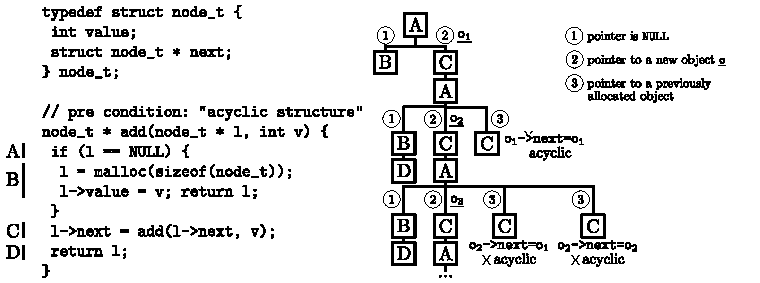
\includegraphics[width=0.9\columnwidth]{images/lazy-initialization} 
  \caption{Example of lazy initialization}
  \label{fig:example-lazy-initialization}
  \vspace{-3mm}
\end{figure*}

\mytempedit{
\boxedexample{
% For the sake of simplicity, we assume that fragment C does not actually evaluate {\tt l->next}, but leaves this task to fragment A. When expanding the [...]
 Figure~\ref{fig:example-lazy-initialization} shows a recursive function {\tt add}, which appends a node of type {\tt node\_t} to a linked list, and a minimal representation of its symbolic execution when applying lazy initialization. The tree nodes represent executions of straight-line fragments of {\tt add}. Initially, fragment A evaluates the value of pointer {\tt l}, which is symbolic and thus uninitialized. The symbolic engine considers three  options: (1) {\tt l} is {\tt NULL}, (2) {\tt l} points to a new object, and (3) {\tt l} points to a previously allocated object. Since this is the first time that a pointer of type {\tt node\_t} is met, option (3) is ruled out. The two remaining options are then expanded, executing the involved fragments. While the first path ends after executing fragment B, the second one implicitly creates a new object {\tt o$_\texttt{1}$} due to lazy initialization and then executes C, recursively invoking {\tt add}. When expanding the recursive call, fragment A is executed and the three options are again considered by the engine, which forks three distinct paths. Option (3) is now taken into account since a {\tt node\_t} object has been previously allocated (i.e., {\tt o$_\texttt{1}$}). However, this path is soon aborted by the engine since it violates the acyclicity precondition (expressed as a comment in this example). The other forked paths are further expanded, repeating the same process. Since the linked list has an unknown maximum length, the exploration can proceed indefinitely. For this reason, it is common to assume an upper bound on the depth of the materialization (i.e., field instantiation) chain.
}
}
% \boxedexample{Consider the C function {\tt add} shown in Figure~\ref{fig:example-lazy-initialization}. This recursive function appends a node of type {\tt node\_t} to the tail of a linked list. A compact representation of the symbolic tree for {\tt add} when applying lazy initialization is given in Figure~\ref{fig:example-lazy-initialization}. Tree nodes A, B, C, and D represent execution of straight-line fragments of code in {\tt add}. Initially, fragment A evaluates the value of the pointer {\tt l}, which is symbolic and thus uninitialized. The symbolic engine considers the three possible options: (1) {\tt l} is {\tt NULL}, (2) {\tt l} points to a new object of type {\tt node\_t}, and (3) {\tt l} points to a previously allocated object. Since this is the first time that a pointer of type {\tt node\_t} is met, option (3) is not considered. The two remaining options are then expanded, executing the required fragments. While the first path ends after executing fragment B, the second path implicitly creates a new object {\tt o$_\texttt{1}$} due to lazy initialization and then executes C, recursively invoking the {\tt add} function. For the sake of simplicity, we assume that fragment C does not actually evaluate {\tt l->next}, but leaves this task to fragment A. Expanding the recursive call, fragment A is executed and the three options are again considered by the engine, forking into three distinct paths. In this case, option (3) is taken into account since an object of type {\tt node\_t} has been previously allocated (i.e., {\tt o$_\texttt{1}$}). However, this forked path is soon aborted by the engine since it violates the acyclic precondition (which is simply expressed as a comment in this example). The other forked paths are further expanded, repeating the same process. Since the linked list has an unknown maximum length, the exploration can proceed indefinitely. For this reason, it is common to assume an upper bound on the depth of the materialization chain.}

\mytempedit{
Recent advances in the area have focused on improving efficiency in generating heap configurations. For instance, in~\cite{DLR-ASE12} the concretization of a reference variable is deferred until the object is actually accessed. The work also provides a formalization of lazy initialization. \cite{BLISS-TSE15} instead employs bound refinement to prune uninteresting heap configurations by using information from already concretized fields, while a SAT solver is used to check whether declarative -- rather than imperative as in the original algorithm -- preconditions hold for a given configuration.
%Further refinements to lazy initialization are described in a number of works, e.g.,~\cite{DLR-ASE12,BLI-NFM13,BLISS-TSE15}. \cite{DLR-ASE12} besides providing a formalization of this technique, extends lazy initialization by adding support for subtypes and by deferring even further concretization when possible (e.g., a check for nullity does not always imply immediate materialization for an object). \cite{BLI-NFM13} presents {\em bounded lazy initialization} (BLI), which exploits {\em tight field bounds}~\cite{GRP-ISSTA10} to prune unfeasible heap configurations. BLISS~\cite{BLISS-TSE15} extends BLI by integrating two techniques: {\em bound refinement} and {\em satisfiability checks}. The former prunes uninteresting heap configurations by leveraging information from already-concretized fields, while the latter queries a SAT solver to check declarative preconditions, discarding unrealistic heap configurations.
}

%, which all share the goal of reducing the number of heap configurations to generate when forking the state. extends lazy initialization by handling subtypes and by making the approach even more lazier, provides a formal treatment of lazy initialization in Java.

\iffullver{
\mytempedit{\myparagraph{Verifying Client Code Only}}
Of a different flavor is the technique presented in~\cite{SHZ-TAIC07} for symbolic execution over objects instantiated from commonly used libraries. The authors argue that performing symbolic execution at the representation level might be redundant if the aim is to only check the client code, thus trusting the correctness of the library implementation. They discuss the idea of symbolically executing methods of the Java {\tt String} class using a finite-state automaton that abstracts away the implementation details. They present a case study of an application that dynamically generates SQL queries: symbolic execution is used to check whether the statements conform to the SQL grammar and possibly match injection patterns. \iffullver{The authors mention that their approach might be used to symbolically execute over standard container classes such as trees or maps. It is worth mentioning that symbolic execution is used to detect SQL injection vulnerabilities also in~\cite{FLP-COMPSAC07}.}{The authors mention that their approach might be used to symbolically execute over standard container classes such as trees or maps.}
}{}

%% citations for SL tools omitted
% Several tools based on SL are available to date for automatically finding memory bugs in user~\cite{INFER} and system-level code~\cite{SLAYER-CAV11}, and for verifying annotated programs with respect to, e.g., memory safety properties~\cite{VERIFAST-APLAS10} and design patterns~\cite{JSTAR-OOPSLA08}. While tailor-made theorem provers are implemented in many extant tools, recent works~\cite{BPS-ENTCS09,PWZ-CAV13}

% While some of them implement tailor-made theorem provers, it has been shown~\cite{BPS-ENTCS09,PWZ-CAV13} that provers for decidable fragments of SL can be integrated in an SMT solver, allowing for complete combinations with other theories relevant for program verification. This paves the way for interesting applications of SL in general-purpose verification tools. In particular, symbolic executors could use it to reason inductively over manipulations of data structures such as lists and trees in C and Java programs. To the best of our knowledge, while symbolic execution is at the core of SL, there have not been applications of SL in symbolic executors yet. We believe this might represent a promising research direction to follow.


% Additional optimizations are presented in~\cite{DLR-ASE12}, which also provides a complete formalization of this approach for the Java language.

% [D] this is related to input test generation
%Also, generated heap configurations are pairwise non-isomorphic: eliminating symmetric structures can greatly reduce the number of heaps that a symbolic executor must explore, while guaranteeing that no relevant states are missed~\cite{BLISS-TSE15}. 

%~\cite{KPV-TACAS03,SPF-ISSTA04} combine lazy initialization with user-provided {\em method preconditions}, i.e., conditions which are assumed to be true before the execution of a method. Such conditions are used to characterize those input states in which the method is expected to behave as intended by the programmer. For instance, we expect a binary tree data structure to be acyclic and with every node - except for the root - having exactly one parent. Conservative method preconditions are used to ensure that incorrect structures are eliminated during initialization, speeding the symbolic execution process up.

%Further refinements to lazy initialization are described in a number of works. \cite{BLI-NFM13} introduces {\em bounded lazy initialization} (BLI) to reduce the number of alternatives to explore using available field bounds expressed in TACO, a tool for SAT-based bounded verification of JML-annotated Java code. ~\cite{BLISS-TSE15} presents two novel techniques that build upon BLI. The first technique refines field bounds by leveraging information from already-concretized fields; the technique is then extended by  auxiliary satisfiability checks to determine the feasibility of partially symbolic structure.
